\section{Analysis of the emerged languages}
\label{sec:analysis_language}
In the above experiments, only three configurations lead to success, where a language emerged that the agents used to exchange information: languages with vocabulary sizes of $|V| = 10$, $|V| = 13$ and $|V| = 100$.
They will be referred to as $Lang_{10}$, $Lang_{13}$ and $Lang_{100}$ respectively.
In this section, these three emerged languages is analyzed in more detail.
This is done in two parts.
The first part is a qualitative analysis, to understand, which symbols are used to transfer which information.
In the second part, the emerged languages are compared to English.
More specifically, it is tested if the messages of the sender align with English referring expressions of the target object.

\begin{figure}[ht]
    \centering
    \subfigure[$Lang_{10}$]{
        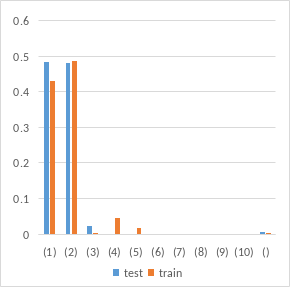
\includegraphics[width=0.31\linewidth]{figures/relative_frequencies_v10.png}
        \label{fig:relative_frequencies_v10}
    }
    \subfigure[$Lang_{13}$]{
        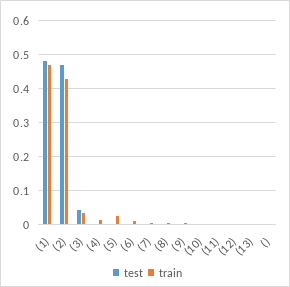
\includegraphics[width=0.31\linewidth]{figures/relative_frequencies_v13.png}
        \label{fig:relative_frequencies_v13}
    }
    \subfigure[$Lang_{100}$, (13 most frequent messages)]{
        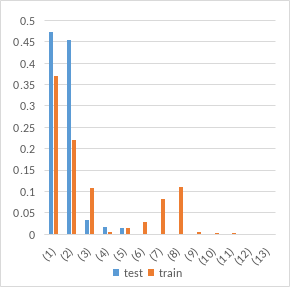
\includegraphics[width=0.31\linewidth]{figures/relative_frequencies_v100.png}
        \label{fig:relative_frequencies_v100}
    }
    \caption{Relative frequencies of messages (ordered by frequency in test dataset)}
    \label{fig:relative_frequencies_vocabularies}
\end{figure}

When looking at the emerged vocabulary \textbf{qualitatively}, a few properties can be seen.
Figure \ref{fig:relative_frequencies_vocabularies} shows an overview of the frequencies of messages in all three emerged languages for the training and the test split.
% SD: I don't understand how test and training set are used in these experiments. In language games one only has a training set and success is measured through the success in the game. It is not possible to have a test set as learning is continuous.
% DK: TODO
Since the tokens themselves are arbitrary, they are ordered by the relative frequency in the messages for the test set and indices for the tokens are added from index 1 for the most frequent token and index $|V|$ for the least frequent token.
By this the languages are easier comparable across different runs and vocabulary sizes.
% SD: I don't understand this.
% DK: TODO
Figure \ref{fig:relative_frequencies_v100} shows only the 13 most frequent message to provide a better overview.
The lesser frequent messages are never used for the test data and each only used one or two times in the train data.

The first property is that when a message is transferred, it consists of only one symbol.
% SD: Is this controlled by the sender. The sender must have some policy how it is assigning messages. Or is it just random? But what makes the sender then to generate a single message vs a longer message. If it is not controlled - how could we implement some policies for message length?
% DK: what do you mean by policy? The sender is only controled by the success of the receiver. If a longer message leads to a better success, it learns to prodcue longer messages. TODO
In some rare cases, also an empty message is communicated.
The models therefore don't learn any compositionality by combining symbols to create new meaning, but rather encode everything in separate symbols.
Secondly, in all three languages, only very few symbols occur with a high frequency, while most of the symbols are used very rarely.
More specifically, two symbols are used in 95\% of the images with $Lang_{10}$ and $Lang_{13}$, while three symbols are used with $Lang_{100}$.
Thirdly, the agents make use of fewer symbols, when presented with unseen test images compared to when communicating about images in the training split.
This is especially visible for $Lang_{100}$.
Symbols that are used for 16,5\% of the training sample are not used at all in test split.
Furthermore, the frequencies in the test split is much more focused on the two most frequent symbols, while it is more distributed around 5 symbols in the train split.
% SD: A table or a graph with these figures?
% DK: is part of the existing figure. The sum of the first two columns (QUESTION)
% SD: Differences between training and testing configuration; what happens during testing, there is no learning involved but the systems see new images but they have to use the same vocabulary?
% DK: exactly

These findings indicate that referring expressions do emerge in each of the newly emerged languages since the agents are able to communicate the correct object.
However, the agents converge towards very few different referring expressions that are made up differently than in English and likely don't rely on the high level attributes \emph{shape}, \emph{color} and \emph{size}.
% SD: Are they? We haven't tested how humans would describe these scene. I see what you mean, but they you have to explain that you count as an English expression a description containing sequences of colour, size and type and then following the Dale and Reiter's algorithm.
% DK: TODO
The similar frequencies across all three languages suggest that a greater vocabulary size $|V|$ doesn't necessarily lead to different referring expressions, but the languages still converge towards two main expressions.
% SD: All this has to do with the sender's policty how to generate messages. We should have varied this policy. I suspect no policy leads just to one message. How is the system motivated to generate more than one symbol?
% DK: TODO

\begin{figure}[ht]
    \centering
    \subfigure[$Lang_{10}$]{
        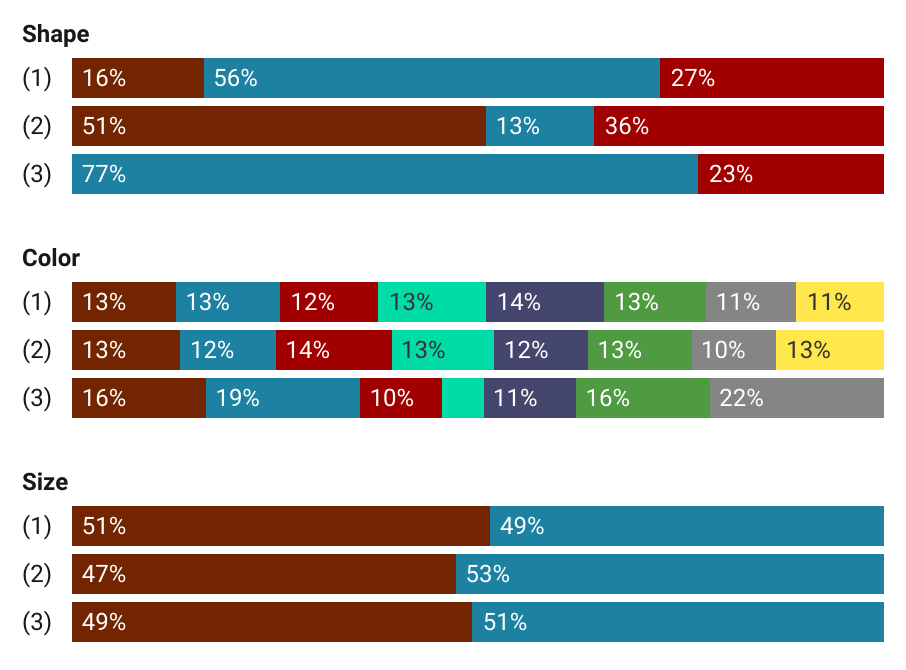
\includegraphics[width=0.31\linewidth]{figures/language_analysis_v10.png}
        \label{fig:language_analysis_v10}
    }
    \subfigure[$Lang_{13}$]{
        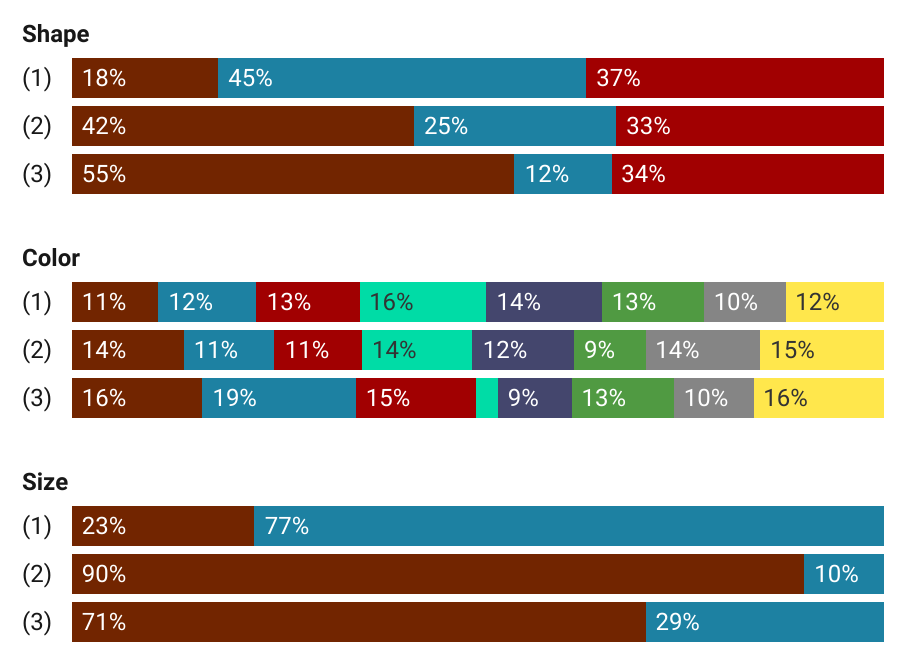
\includegraphics[width=0.31\linewidth]{figures/language_analysis_v13.png}
        \label{fig:language_analysis_v13}
    }
    \subfigure[$Lang_{100}$]{
        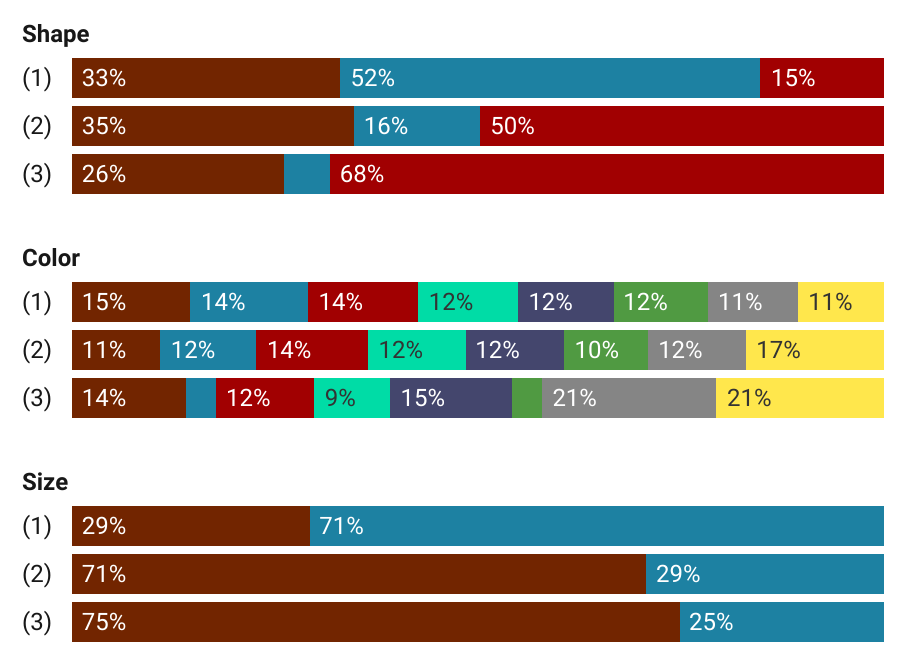
\includegraphics[width=0.31\linewidth]{figures/language_analysis_v100.png}
        \label{fig:language_analysis_v100}
    }
    \caption{Relative share of the described target object's attributes for the top three messages}

    \textbf{Shape:} brown: sphere, blue: cube, red: cylinder \\
    \textbf{Size:} brown: small, blue: large
    \label{fig:language_analysis_vocabularies}
\end{figure}

Figure \ref{fig:language_analysis_vocabularies} shows the attributes of the target object that are described by each message.
Hereby, the relative share each value of all three attributes are displayed.
For instance the first bar in Figure \ref{fig:language_analysis_v10} shows that 16\% of the target objects that are described with symbol (1) in the language $Lang_{10}$ are spheres.
In the figures, only the three most frequently used messages are included, which make up over 95\% of all messages.

The first thing that can be seen is that different symbols convey different values of attributes.
In the language $Lang_{10}$, symbol (1) is mostly used for target objects that are cubes, while symbol (2) is mostly used for spheres.
There is not much difference for target objects that are cylinders.
The distribution for colors is almost constant across symbols (1) and (2).
Symbol (3) is more frequently used for blue, green and gray objects, while being less used for red, cyan and yellow objects.
This different distribution may also be caused by the much lower absolute usage of symbol (3).
The different sizes are encoded by all symbols in the same way.

Looking at $Lang_{13}$ the symbol usage differs.
The frequencies for the shape look similar, but (the much less used) symbol (3) encodes most of the time spheres instead of cubes.
Again, the colors look similar with small deviations for brown, green and yellow objects.
Most striking however, is the difference for the size.
Symbol (1) is used in 77\% of the cases for large objects, while symbol (2) and (3) are used in 90\% and 71\% of the messages for small objects.

Language $Lang_{100}$ uses symbols its symbols to discriminate cubes and cylinders, while the frequencies for sphere remain constant across all symbols.
The usage for the color is similar to $Lang_{13}$.
Looking at the size, as for $Lang_{13}$, symbol (1) is mostly used to encode small objects, while symbols (2) and (3) are mostly used to encode large objects.

An interesting observation is that symbols are not used for the same attributes across the languages.
In some languages, an attribute is not captured at all by the symbols, while another language heavily relies on it.
The same applies to the values of attributes, especially to the shapes.
Only two of the shapes are distinguished by the usage of symbols, while the third is not captured.
Which shape are encoded, differs from language to language.

Furthermore, these numbers confirm even more that the agents don't rely solely on the human defined attributes.
For instance $Lang_{10}$ only encodes the shape in its symbols.
This would not be enough to distinguish the target object from the distractor consistently.
Following, the agents also encode some additional underlying attributes and patterns to the three above defined attributes.
% SD: But this is slightly problematic, since we strcutured the world this way to emphasise these attributes visually. Hence, a mapping would indicate that the symbols have good semantics if they can discriminate the colours. But this could have to do with the compisitionality issue, perhaps the system was biased to use single word expressions and hence this interfered with the grounding.
% DK: TODO

To compare the emerged language to English in a \textbf{quantitative} way, a probing approach is used.
Probing can be used to analyze and interpret the hidden representations in neural networks.
Hereby, a second neural model is trained to predict selected linguistic properties on the basis of the hidden representations.
If this model is successfully able to predict the linguistic properties, the hidden representations are connected to them.
If second model can't be trained, it indicates that there is no correlation between the hidden representation and the linguistic property.
In the case of the emerged language, a neural model is trained to translate the messages of the sender into English referring expressions, based on the GRE algorithm by \citet{Dale1995}.
% SD: The probing test is to show how well the emerged language can be trasnlated into English descriptions consistting of labels of scene features using Dale and Reiter idea of incrementality. However, we would need to know now what was the policy of the sender to generate message. Was this similar to Dale and Reiter to enforce longer descriptions?
% DK: TODO
Hereby, the model consists of an encoder LSTM, one linear layer and a decoder LSTM.
The encoder LSTM encodes the messages of the emerged language.
The final hidden state is used as the meaning of the complete sentence and passed through the linear layer, which should learn an abstract representation of the message.
The resulting vector is used as the initial state of the decoder LSTM.
The decoder LSTM is then trained to produce the English referring expression.
While decoding, teacher forcing is applied.
The success of the model is validated calculating cross entropy between the models predictions and the target English referring expression.
Since generalization doesn't play a role for probing, no dropout is applied and the model is trained and validated on the complete dataset; no test or validation split is used.

In the sections above, the attributes are ordered by importance in the way, it is usually used in English: shape > color > size.
Since the agents do not necessarily need to follow this, all possible orders of importance for the attributes are compared to each other.
% SD: Move to the earlier paragraph when you introduce Dale and Reiter.
% DK: TODO

The translation model with this setup can learn two characteristics.
First, it can learn to find correlations between the emerged language and the English referring expressions.
Secondly, it can learn patterns in the English referring expressions that are independent of the emerged language.
For instance, it can learn that the referring expressions are likely to be two symbols long, or that 'cube' is the most common shape.
This second characteristic can lead to a low loss of the model, even though there are no connections to the emerged language.
In this test, only the first characteristic is interesting and would show the correlation between the emerged language and English referring expressions.
For that reason, two reference baselines are calculated for each of the attribute importance order.
% SD: Baselines?
% DK: (done)
The first reference uses a non-informative input for the encoder LSTM, more specifically it always receives a vector of zeros and therefore can't learn any meaningful representation in the linear layer; the input for the decoder LSTM is the same for every sample.
By this, the model is trained to learn the patterns in the English referring expressions.
The resulting loss is the highest possible loss the model can achieve, independent of the input.
Resulting, if the emergent language is connected to English, the loss will be lower than this baseline.
If not, the loss will be as high as this baseline.
On the other side, we calculated the lowest loss possible, by using the English referring expressions as both input and target.
This verifies that the model is able to learn an abstract representation from the input and the resulting loss should be close to zero (since input is perfectly correlated to the target).
These two references are used, to normalize the results of the actual emergent languages $L_{em}$, using the formula $L_{norm} = \frac{L_{em}-L_{English}}{L_{baseline} - L_{English}}$.
A loss close as $L_{baseline}$ will lead to 100\%, while a loss as $L_{English}$ will lead to 0\%.
% SD: Is this encessary? But when and where is this loss using 0 inouts calculated?
% DK: TODO, QUESTION
By doing this, all configurations can be compared directly to each other.

\begin{table}[ht]
    \centering
    \begin{tabular}{c|cc|cc|cc|cc}
        \toprule
        \textbf{Order}          & $L_{baseline}$ & $L_{English}$ & \multicolumn{2}{c}{$|V| = 10$} & \multicolumn{2}{c}{$|V| = 13$} & \multicolumn{2}{c}{$|V| = 100$}                                                      \\\cmidrule(lr){4-5}\cmidrule(lr){6-7}\cmidrule(lr){8-9}
                                &                &               & $L_{em}$                       & $L_{norm}$                     & $L_{em}$                        & $L_{norm}$         & $L_{em}$ & $L_{norm}$         \\\midrule
        {shape > color > size}  & {0,659}        & {0,0001}      & {0,569}                        & \textbf{86,19\%}               & {0,622}                         & {94,24\%}          & {0,597}  & {90,4\%}           \\
        {shape > size > color}  & {0,589}        & {0,0002}      & {0,489}                        & \textbf{83,09\%}               & {0,531}                         & {90,21\%}          & {0,47}   & {\textbf{79,78\%}} \\
        {color > shape > size}  & {0,849}        & {0,0}         & {0,802}                        & 94,49\%                        & {0,801}                         & {94,36\%}          & {0,791}  & {93,15\%}          \\
        {color  > size > shape} & {0,836}        & {0,0}         & {0,819}                        & 98,01\%                        & {0,772}                         & {92,35\%}          & {0,786}  & {94\%}             \\
        {size > shape > color}  & {0,532}        & {0,0052}      & {0,492}                        & 92,26\%                        & {0,437}                         & {\textbf{81,95\%}} & {0,457}  & {\textbf{85,61\%}} \\
        {size > color > shape}  & {0,599}        & {0,0001}      & {0,573}                        & 95,71\%                        & {0,495}                         & {\textbf{82,67\%}} & {0,538}  & {\textbf{89,87\%}} \\
        \bottomrule
    \end{tabular}
    \caption{Cross entropy losses while probing with emerged languages successful on 'Dale-2'}
    % SD: I have a trouble of understanding and interpreting these results. First the loss should be estimated on a test set, after the system has been trained. I'm not sure how you estaimate the baseline loss.
    % DK: TODO, why a test set? Isn't the purpose to learn how well the generated captions map to English and not how well they generalize. Using only the train set exactly shows if a mapping is possible
    \label{tab:probing_discrimnator_language}
\end{table}

Table \ref{tab:probing_discrimnator_language} shows the results for all different languages.
First, it can be seen for all emerged languages, the model is able to find correlations between natural language referring expressions and the messages by the sender.
Still, all losses stay high and closer to the loss of the baseline, namely where the model only learns the patterns in the English referring expressions.
This fact concludes that all emerged languages don't rely on the GRE algorithm by \citet{Dale1995}.
Nonetheless, it may be possible that a different algorithm is used to create referring expressions in the artificial language.
% SD: I think at this point a readerwill be confused since we are discussing Dale and Reiter bith for generation of scenes and now for the generation of strings. We should have clarified the difference earlier. Also, rather than referring to it as Dale and Reiter we should call it "the incremental algorithm" and add a reference at first mention.
% DK: TODO

Secondly, it can be seen that the correlation between the emerged language and the natural language referring expressions differ for each of the languages.
The vocabulary consisting of 10 symbols is the closest related to the orders \emph{shape > size > color} and \emph{shape > color > size}, the vocabulary based on 13 symbols on the other hand to the orders \emph{size > shape > color} and \emph{size > color > shape}.
With 100 symbols, the vocabulary resembles mostly \emph{shape > size > color} and \emph{size > shape > color}.
Striking here is that even though the related orders are different, the most important attributes are either the \emph{size} or \emph{shape} across all three emerged languages.
The attribute \emph{color} seems to be less important.
This is reinforced by the fact that the losses are closer to the baseline, when the \emph{color} is the most or second most important attribute in the order.
